% Sample extended abstract. Port the body into the Moodle template before submission.
% Red \TBD{...} marks results that do not exist yet: replace every one with the real number or sentence.
\documentclass[10pt,twocolumn]{article}
\usepackage[a4paper,margin=0.62in,columnsep=0.22in]{geometry}
\usepackage[T1]{fontenc}
\usepackage{mathptmx}
\usepackage{amsmath,amssymb}
\usepackage{graphicx}
\usepackage{booktabs}
\usepackage{xcolor}
\usepackage{caption}
\usepackage[round]{natbib}
\usepackage[hidelinks]{hyperref}
\captionsetup{font=small,labelfont=bf,skip=3pt}
\setlength{\textfloatsep}{8pt plus 2pt}
\setlength{\floatsep}{6pt plus 2pt}
\setlength{\abovedisplayskip}{3pt}\setlength{\belowdisplayskip}{3pt}
\setlength{\parskip}{0pt}
\newcommand{\TBD}[1]{\textcolor{red}{\textbf{[#1]}}}
\newcommand{\BA}{\mathrm{BA}}
\makeatletter
\renewcommand\section{\@startsection{section}{1}{\z@}{-5pt plus -1pt}{2pt}{\normalfont\large\bfseries}}
\renewcommand\subsection{\@startsection{subsection}{2}{\z@}{-3pt plus -1pt}{1pt}{\normalfont\normalsize\bfseries}}
\makeatother

\title{\vspace{-0.9cm}\textbf{Reading Both Halves of \emph{Imvo}: What Modernising 1880s isiXhosa\\ Does to Cross-Lingual Analysis}\vspace{-0.25cm}}
\author{Lily de Melo \quad Tawananyasha Kadango \quad Sally Mohlakola\\ {\small University of the Witwatersrand}}
\date{\vspace{-0.9cm}}

\begin{document}
\maketitle

\section{Introduction}
\emph{Imvo Zabantsundu}, founded by John Tengo Jabavu in 1884, was the first African-owned and run
newspaper in South Africa \citep{schoots}. It was written mainly in isiXhosa, but also printed an English
translation of the editorial and, at times, other English articles, letters and advertisements
\citep{schoots}. In the text files we use, 511 of 517 issues from 1884--1894 contain at least 1{,}000
words in each language. Each issue therefore addressed two readerships under one editor.
Because NLP tools are far stronger for English than for isiXhosa, it is tempting to analyse the English
half alone, or to ``clean'' the isiXhosa half first. One such step is \emph{spelling modernisation}: the archive writes \emph{Tixo}, \emph{apa} and \emph{umteto} where modern
isiXhosa writes \emph{Thixo}, \emph{apha} and \emph{umthetho}. It is tempting to treat modernisation as
neutral preprocessing. We test that assumption.

\textbf{Research question.} \emph{When Imvo's isiXhosa and English sections from the same issue are
placed in one multilingual embedding space, how distinguishable is their content, and how does
modernising the isiXhosa spelling change that answer?}
\textbf{H1:} once language identity is removed, a classifier predicts a chunk's section above a
\emph{translated-pair floor}, i.e.\ the audiences received different content.
\textbf{H2:} modernisation lowers the floor (less spelling signal) but leaves the content gap unchanged;
a significant change in the gap would mean modernisation alters the substantive conclusion.
\textbf{Contributions:} (i) a variant of linear language-subspace removal \citep{lir} that estimates the
subspace only from translated pairs, so that genuine content differences are not removed with it,
validated on synthetic data with a known answer; (ii) a lexicon-gated normaliser with rule ablations; (iii) a
measurement of what modernisation changes, including which names it rewrites.

\section{Background and related work}
The isiXhosa Intellectual Traditions archive digitised isiXhosa newspapers from 1870--1894. Every page was
OCR-corrected by first-language isiXhosa speakers, and the text was deliberately not spell-checked,
because the orthography of the period differs from present-day isiXhosa \citep{schoots}.
Historical text normalisation maps old spellings to modern ones and is usually evaluated by
normalisation accuracy or downstream task scores \citep{bollmann}, not by whether it changes the
conclusions drawn from the text. Multilingual sentence encoders such as LaBSE \citep{labse} embed many
languages, including isiXhosa, in one space, but their representations still encode language identity.
It can be removed by subtracting each language's mean \citep{libovicky} or by projecting out a low-rank
language subspace \citep{lir}; iterative nullspace projection removes a protected attribute in a similar
way \citep{inlp}. For a linear probe, mean-centring equalises the two languages' means, so it also removes
genuine average content differences, which is exactly what we want to measure. We therefore estimate the
language subspace from translated pairs only. Treating modernisation as a choice that can change
results follows the ``garden of forking paths'' view of analytic flexibility \citep{gelman}.

\section{Method}
\textbf{Data.} We use the archive's language-split text for 511 of 517 Imvo issues (1884--1894) that
contain $\geq$1{,}000 words in each language (3.9M isiXhosa and 1.5M English words before filtering, close
to the archive's own counts of 4.0M and 1.5M for all of Imvo \citep{schoots}). We repair only layout and
OCR artefacts such as words hyphenated across lines (never spelling), cut pages into 60-word chunks, and flag boilerplate (a chunk is flagged if
$\geq$30\% of its 5-word sequences recur in $\geq$5 issues: adverts, notices, tax lists) and chunks whose
language does not match their section. This leaves 45{,}465 isiXhosa and 22{,}927 English chunks.
Issues are split 357/77/77 into train/validation/test, stratified by year, so no issue crosses splits.
Boilerplate is far more common in the isiXhosa half (29.9\% vs 7.9\%).

\textbf{Modernisation.} From 3.3M tokens \TBD{verify against build\_lexicon.py output} of modern
isiXhosa (Vukuzenzele \citep{vuk}, isiXhosa Wikipedia, OPUS-100 \citep{opus}) we build a word-frequency
list $f(\cdot)$. Two rule families can be switched on separately. \emph{Aspiration} restores unwritten
aspiration ($t,p,k,r$ and clicks $c,q,x$ $\to$ $+h$), trying every combination of eligible positions:
a word $w$ is rewritten to its most frequent variant $w'$ only if $f(w)\le\tau_o$ and $f(w')\ge\tau_v$.
\emph{Prefix} joins prefixes written apart: before a lowercase word only if the joined form has
$f\ge\tau_v$ and is at least five times as frequent as the bare word; before a capitalised word
(\emph{e Palamente} $\to$ \emph{ePalamente}) always, without a word-list gate. $(\tau_o,\tau_v)$ are
chosen to maximise $F_{0.5}$ on hand-checked validation words, since over-correcting an author's
spelling is the costlier error; until those labels exist we use $(\tau_o,\tau_v){=}(2,5)$
\TBD{replace with tuned values}.

\textbf{Embedding and pairs.} Chunks are embedded with LaBSE \citep{labse} (and with multilingual-E5
\citep{e5} as a robustness check). Within each issue, mutual nearest neighbours across the two sections
are candidate translations. We keep candidates with LaBSE similarity $\ge$0.55, a provisional threshold
\TBD{replace with the lowest threshold whose precision is $\ge$0.9 on hand-labelled validation
candidates}. E5 similarities fall in a narrow band (0.83--0.87), so E5 needs its own threshold.

\textbf{Removing language, measuring content.} Let $P$ be the translated pairs in training issues.
Because a pair shares its content, its difference is language:
\begin{equation}
D=\big[\,x^{\mathrm{xh}}_i-x^{\mathrm{en}}_i\,\big]_{i\in P},\quad
\tilde{x}=x-V_k^{\top}V_k\,x,
\end{equation}
where $V_k$ holds the top-$k$ right singular vectors of $D$. A balanced logistic-regression classifier
then predicts each chunk's section from $\tilde{x}$. Its balanced accuracy on held-out translated pairs
is the \emph{floor} (language signal that survives); the content gap is
\begin{equation}
\Delta=\BA_{\mathrm{all}}-\BA_{\mathrm{pairs}}.
\end{equation}
$k\in\{0,1,2,4,\dots,64\}$ is the smallest value whose validation floor is $\le$0.55, and the
regularisation $C\in\{0.01,0.1,1,10\}$ is tuned on validation. For H2, modernised variants reuse the raw run's pairs and $k$, so only the
text changes. We report differences with paired bootstrap 95\% CIs over test issues ($B{=}1000$).
Alignment across variants is measured on \emph{embedding-free} pairs (mutual best matches on shared names
and numbers, \TBD{hand-verified}), because pairs selected in the raw space would favour raw by construction.

\textbf{Validation.} On synthetic data with a planted content gap, we compare our method with no
removal and with mean-centring against an oracle that sees content only.

\section{Results}
\textbf{The method recovers known gaps.} On synthetic data, without language removal the classifier
separates translated pairs perfectly (floor 1.00, gap 0): it detects language, not content.
Mean-centring reports a gap of 0.000 at every effect size, as expected for a linear probe once the
class means are equal. The pair-based method tracks the oracle closely (Fig.~\ref{fig:syn}; at
$\delta{=}0.4$: 0.097 vs 0.099).

\begin{figure}[t]
\centering
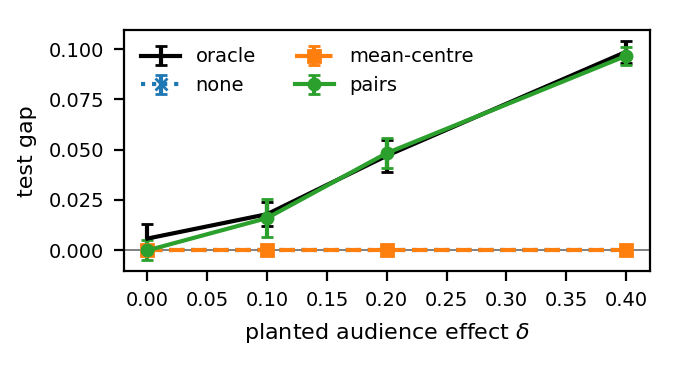
\includegraphics[width=0.92\columnwidth]{figures/fig_synthetic.png}
\caption{Synthetic validation (5 seeds per effect size $\delta$; error bars = s.d.). Only the
pair-based method recovers the oracle content gap; mean-centring erases it.}
\label{fig:syn}
\end{figure}

\textbf{What modernisation changes.} With provisional thresholds ($\tau_o{=}2,\tau_v{=}5$), the full
normaliser rewrites 12.4\% of the 3.7M alphabetic isiXhosa tokens: aspiration 7.8\% (e.g.\ \emph{apa}$\to$\emph{apha},
\emph{pakati}$\to$\emph{phakathi}, \emph{ipepa}$\to$\emph{iphepha}) and prefix joining 4.6\%.
\TBD{Normaliser precision/recall on held-out words, from normalise.py tune.} The aspiration rule alone
rewrites 149 likely proper names (capitalised in $\ge$90\% of occurrences; 12{,}966 tokens), including \emph{Xosa}$\to$\emph{Xhosa},
\emph{Tembu}$\to$\emph{Thembu}, \emph{Mtata}$\to$\emph{Mthatha} and \emph{Tixo}$\to$\emph{Thixo}.
Table~\ref{tab:tools} shows that modernisation mainly changes vocabulary: 31.5\% of raw word tokens are
absent from modern text, against 24.5\% after restoring aspiration, while subword fertility barely moves.
Prefix joining alone raises OOV to 34.2\%, consistent with its joins before capitalised words not
being checked against the word list.

\begin{table}[t]
\centering\small
\caption{How modern tools see the text. OOV = share of word tokens absent from the modern word list;
fertility = subword tokens per raw word.}
\label{tab:tools}
\begin{tabular}{@{}lccc@{}}
\toprule
Text & OOV & LaBSE & XLM-R \\
\midrule
Imvo isiXhosa, raw & 31.5\% & 2.11 & 2.50 \\
\quad + aspiration only & 24.5\% & 2.09 & 2.51 \\
\quad + prefix joining only & 34.2\% & 2.14 & 2.51 \\
\quad + both (modern) & 26.8\% & 2.12 & 2.52 \\
Imvo English & -- & 1.26 & 1.38 \\
Modern isiXhosa (Vukuzenzele) & -- & 2.18 & 2.92 \\
\bottomrule
\end{tabular}
\end{table}

\textbf{Two audiences (H1) and the effect of modernisation (H2).}
Table~\ref{tab:main} and Fig.~\ref{fig:main} report the section classifier on test issues
(\TBD{$n$} reference pairs, $k{=}$\TBD{k}). \TBD{One sentence on H1: is $\Delta_\mathrm{raw}>0$ with a CI
excluding 0?} \TBD{One sentence on H2: how floor and $\Delta$ move under each variant.}

\begin{table}[t]
\centering\small
\caption{Section classifier (test balanced accuracy) and alignment. $\Delta$ = all $-$ floor;
brackets: paired bootstrap 95\% CI of the change vs raw. P@1 on embedding-free true pairs.}
\label{tab:main}
\begin{tabular}{@{}lccccc@{}}
\toprule
Variant & All & Floor & $\Delta$ & $\Delta-\Delta_\mathrm{raw}$ & P@1\\
\midrule
raw & \TBD{} & \TBD{} & \TBD{} & -- & \TBD{}\\
modern & \TBD{} & \TBD{} & \TBD{} & \TBD{CI} & \TBD{}\\
aspiration only & \TBD{} & \TBD{} & \TBD{} & \TBD{CI} & \TBD{}\\
prefix only & \TBD{} & \TBD{} & \TBD{} & \TBD{CI} & \TBD{}\\
\midrule
E5: modern & \TBD{} & \TBD{} & \TBD{} & \TBD{CI} & \TBD{}\\
\bottomrule
\end{tabular}
\end{table}

\begin{figure}[t]
\centering
\fbox{\parbox[c][3.6cm][c]{0.9\columnwidth}{\centering\TBD{fig\_compare.png from compare.py}}}
\caption{\TBD{Caption stating what the reader should see, e.g.\ the floor falls under modernisation
while $\Delta$ stays within its CI.}}
\label{fig:main}
\end{figure}
In a single-issue pilot, LaBSE already matched genuine translations (an obituary, a magistrate's report,
a franchise petition) at similarity 0.54--0.67, against a median of 0.25 for random pairs.
\TBD{Qualitative: clusters most over-represented in the isiXhosa half (from qualitative.md), with one
short quoted example, and the per-issue JSD vs permutation baseline.}

\section{Discussion}
\textbf{The control is the method.} A naive section classifier scores perfectly and tells us nothing,
and the standard fix (mean-centring) silently assumes the answer to H1 is ``no''. Estimating the
language subspace only from translated pairs separates language from content without that
assumption, and the synthetic check shows it recovers gaps of the size we test for.

\textbf{Modernisation is a forking path.} \TBD{One of: (a) if $\Delta$ is unchanged while the floor
falls: modernisation removes spelling signal but leaves the audience conclusion intact, so it is safe
for this question but not neutral for alignment; or (b) if $\Delta$ changes: the substantive conclusion
about what Imvo told its two audiences depends on a preprocessing choice that is rarely reported.}
Either way, the ablation shows which rule family drives the change, and Table~\ref{tab:tools} explains
why: modernisation acts on vocabulary, not on how text is segmented.

\textbf{What ``fixing'' text costs.} The normaliser rewrites the names of a people (\emph{Xosa}), a
community (\emph{Tembu}), a town (\emph{Mtata}) and God (\emph{Tixo}) into today's forms. These are
correct modern spellings, but they replace how the authors wrote their own names and beliefs. A
digitised archive that silently modernises becomes a different historical record. We therefore
recommend that analyses of historical African-language text report a \emph{normalisation sensitivity}
check: run the analysis on raw and normalised text and report both.

\textbf{Limitations.} Translated pairs are concentrated in some genres \TBD{genre mix of pairs}, and at
the provisional threshold 43\% come from 1885--86, so the floor may not represent all genres or years.
Labelling was done by \TBD{team's isiXhosa reading level}. Prefix joins before capitalised words (4.6\%
of tokens) are applied without a word-list gate or hand-checking. The modern word list is dominated by
OPUS-100 web text \TBD{verify against build\_lexicon.py output}. The archive reports no OCR error rate
\citep{schoots}, so residual OCR noise is unmeasured. We measure differences in content, not editorial
intent.

\clearpage
\small
\begin{thebibliography}{9}\setlength{\itemsep}{0pt}
\bibitem[Bollmann(2019)]{bollmann} M.~Bollmann. A large-scale comparison of historical text normalization systems. \emph{NAACL}, 2019.
\bibitem[Feng et~al.(2022)]{labse} F.~Feng, Y.~Yang, D.~Cer, N.~Arivazhagan, W.~Wang. Language-agnostic BERT sentence embedding. \emph{ACL}, 2022.
\bibitem[Gelman and Loken(2013)]{gelman} A.~Gelman, E.~Loken. The garden of forking paths. Technical report, Columbia University, 2013.
\bibitem[Lastrucci et~al.(2023)]{vuk} R.~Lastrucci, J.~Rajab, M.~Shingange, D.~Njini, V.~Marivate. Preparing the Vuk'uzenzele and ZA-gov-multilingual South African multilingual corpora. \emph{RAIL}, 2023.
\bibitem[Libovick{\'y} et~al.(2020)]{libovicky} J.~Libovick{\'y}, R.~Rosa, A.~Fraser. On the language neutrality of pre-trained multilingual representations. \emph{Findings of EMNLP}, 2020.
\bibitem[Ravfogel et~al.(2020)]{inlp} S.~Ravfogel, Y.~Elazar, H.~Gonen, M.~Twiton, Y.~Goldberg. Null it out: Guarding protected attributes by iterative nullspace projection. \emph{ACL}, 2020.
\bibitem[Schoots et~al.(2023)]{schoots} J.~Schoots, A.~Ngwendu, J.~De~Wet, S.~Muftic. IsiXhosa intellectual traditions digital archive: Digitizing isiXhosa texts from 1870--1914. \emph{RAIL}, 2023.
\bibitem[Wang et~al.(2024)]{e5} L.~Wang et~al. Multilingual E5 text embeddings: A technical report. arXiv:2402.05672, 2024.
\bibitem[Yang et~al.(2021)]{lir} Z.~Yang, Y.~Yang, D.~Cer, E.~Darve. A simple and effective method to eliminate the self language bias in multilingual representations. \emph{EMNLP}, 2021.
\bibitem[Zhang et~al.(2020)]{opus} B.~Zhang, P.~Williams, I.~Titov, R.~Sennrich. Improving massively multilingual neural machine translation and zero-shot translation. \emph{ACL}, 2020.
\end{thebibliography}

\normalsize
\section*{Contribution statement}
We (Lily de Melo, Tawananyasha Kadango and Sally Mohlakola) worked together fairly on this project.
\TBD{paste final contribution statement.}

\section*{AI Ethics Statement}
\TBD{Faculty of Science AI Ethics Statement.}

\section*{NeurIPS Paper Checklist}
\TBD{\textbackslash input the NeurIPS 2024 checklist .tex from Moodle here, filled in.}

\end{document}
